\chapter{Data-Driven Coarsening of Finite Elements}
\section{Background}
\subsection{The Finite Element Method}
The finite element method~\citep{ciarlet2002finite} is a way to numerically approximate solutions to partial differential equations.
The function domain $\Omega$ is divided into a finite number of elements $E_k$.
A polynomial function is defined over each element.
These polynomials form a basis for discrete approximations to the solution.

This thesis uses eight-node hexahedron elements defined in $\mathbb{R}^3$
to perform all of the mechanical analysis.
The eight-node hexahedron element is the simplest of the hexahedron family.
It represents continuous functions supported inside the element by trilinearly interpolating function values defined on its eight nodes.
Each node $\mathbf{X}_i$ resides in $\mathbb{R}^3$ with a given real value $u(\mathbf{X}_i)$.
The nodal positions must cooperate to guarantee that no point inside the hexahedron is inverted.
This will be explained later.
For now, suppose the element shape is well-defined and 
consider a point $\mathbf{X}\in\mathbb{R}^3$ inside the element.
The trilinear interpolation on $\mathbf{X}$ is given by
\[
u(\mathbf{X})=\sum_i w_iu(\mathbf{X}_i),
\]
for some weights $w_i$ that depends on the relative position between $\mathbf{X}$ 
and $\mathbf{X}_i$.

In order to write down the expression for $w_i$, we need to introduce the standard quadrilateral or hexahedral element (Figure~\ref{fig:standardEle}).
The standard hexahedron is just a cube centered at the origin spanning $[-1,1]^3$.
The axis are labeled with $\xi, \eta, \zeta$ to distinguish from the space that $\mathbf{X}$ resides in.
This new coordinate system is known as the isoparametric hexahedral coordinates or more commonly referred to as \textbf{natural coordinates}.
The nodal positions of the standard elements in the natural coordinates are listed in Table~\ref{tab:natCoord}.
For a point $(\xi, \eta,\zeta)$ in the natural coordinates,
its interpolation weights is defined as in Equation~\ref{eq:triWeight}.
\begin{equation}
	w_i=\frac{1}{8}(1+\xi_i\xi)(1+\eta_i\eta)(1+\zeta_i\zeta).
	\label{eq:triWeight}
\end{equation}
Note that the sum of the weights is always $1$ for any point inside the element.
Suppose now we define a ``density'' value of $1$ on each of its eight vertices,
we can compute the total mass of the element by 
\[
mass=\int_{-1}^{1}\int_{-1}^{1}\int_{-1}^{1}\sum_i w_i\cdot 1 \,d\xi \,d\eta\,d\zeta=
\int_{-1}^{1}\int_{-1}^{1}\int_{-1}^{1} 1 \,d\xi \,d\eta\,d\zeta=8.
\]
This is simply the volume of the standard element multiplied by the density.
This partition of unity property of the interpolation function is crucial for physical meanings of quantities defined on the element.
\begin{figure}
\centering
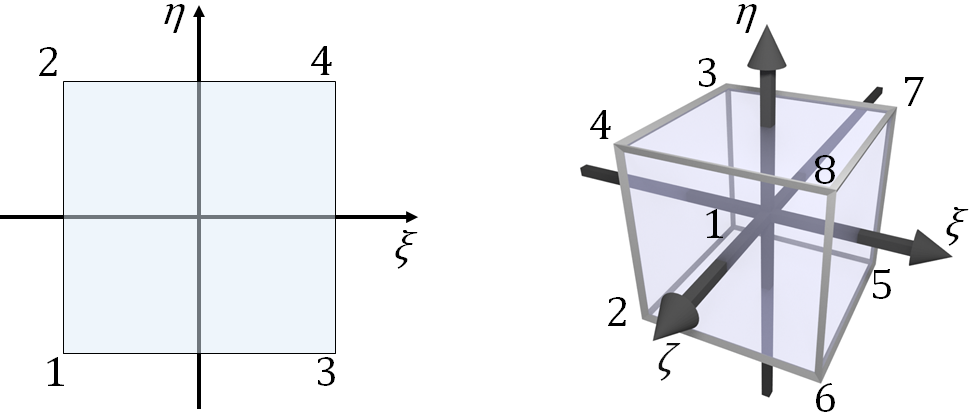
\includegraphics[width=0.8\textwidth]{figs/refEle.png}
\caption{Standard elements for 2D quadrilateral (left) 
	and 3D hexahedral elements (right). The standard element spans $[-1,1]$ in each axis
	to facilitate Gaussian quadrature rules. Nodes are marked with their indices.
	}
\label{fig:standardEle}
\end{figure}
\begin{table}
	\begin{center}
		\begin{tabular}{ |c| r r r|}
			\hline
			Index & $\xi_i$ & $\eta_i$ & $\zeta_i$ \\ \hline
			1 & -1 & -1 & -1\\  
			2 & -1 & -1 & 1\\
			3 & -1 & 1 & -1\\  
			4 & -1 & 1 & 1\\
			5 & 1 & -1 & -1\\  
			6 & 1 & -1 & 1\\
			7 & 1 & 1 & -1\\  
			8 & 1 & 1 & 1\\
		\hline						
		\end{tabular}
	\end{center}
	\caption{Nodal positions of the standard hexahedron element in the natural coordinates.
		Coincidentally, these coordinate values can also be used to define the trilinear interpolation weights.}
	\label{tab:natCoord}
\end{table}

\subsection{Modeling Elastic Objects}

\section{}
